\documentclass[12pt]{article}
\usepackage[left=1cm, right=1cm, top=2cm,bottom=1.5cm]{geometry} 

\usepackage[parfill]{parskip}
\usepackage[utf8]{inputenc}
\usepackage[T2A]{fontenc}
\usepackage[russian]{babel}
\usepackage{enumitem}
\usepackage[normalem]{ulem}
\usepackage{amsfonts, amsmath, amsthm, amssymb, mathtools,xcolor}
\usepackage{blkarray}

\usepackage{tabularx}
\usepackage{hhline}

\usepackage{accents}
\usepackage{fancyhdr}
\pagestyle{fancy}
\renewcommand{\headrulewidth}{1.5pt}
\renewcommand{\footrulewidth}{1pt}

\usepackage{graphicx}
\usepackage[figurename=Рис.]{caption}
\usepackage{subcaption}
\usepackage{float}

%Добавление русской азбуки
\AddEnumerateCounter{\asbuk}{\russian@alph}{щ}

%%Наименование папки откуда забирать изображения
\graphicspath{ {./images/} }

%%Изменение формата для ввода доказательства
\renewcommand{\proofname}{$\square$  \nopunct}
\renewcommand\qedsymbol{$\blacksquare$}

%%Изменение отступа на таблицах
\addto\captionsrussian{%
	\renewcommand{\proofname}{$\square$ \nopunct}%
}
%% Римские цифры
\newcommand{\RN}[1]{%
	\textup{\uppercase\expandafter{\romannumeral#1}}%
}

%% Для удобства записи
\newcommand{\MR}{\mathbb{R}}
\newcommand{\MC}{\mathbb{C}}
\newcommand{\MQ}{\mathbb{Q}}
\newcommand{\MN}{\mathbb{N}}
\newcommand{\MZ}{\mathbb{Z}}
\newcommand{\MTB}{\mathbb{T}}
\newcommand{\MTI}{\mathbb{I}}
\newcommand{\MI}{\mathrm{I}}
\newcommand{\MCI}{\mathcal{I}}
\newcommand{\MJ}{\mathrm{J}}
\newcommand{\MH}{\mathrm{H}}
\newcommand{\MT}{\mathrm{T}}
\newcommand{\MU}{\mathcal{U}}
\newcommand{\MV}{\mathcal{V}}
\newcommand{\MB}{\mathcal{B}}
\newcommand{\MF}{\mathcal{F}}
\newcommand{\MW}{\mathcal{W}}
\newcommand{\ML}{\mathcal{L}}
\newcommand{\MP}{\mathcal{P}}
\newcommand{\VN}{\varnothing}
\newcommand{\VE}{\varepsilon}
\newcommand{\dx}{\, dx}
\newcommand{\dy}{\, dy}
\newcommand{\dz}{\, dz}
\newcommand{\dd}{\, d}


\theoremstyle{definition}
\newtheorem{defn}{Опр:}
\newtheorem{rem}{Rm:}
\newtheorem{prop}{Утв.}
\newtheorem{exrc}{Упр.}
\newtheorem{problem}{Задача}
\newtheorem{lemma}{Лемма}
\newtheorem{theorem}{Теорема}
\newtheorem{corollary}{Следствие}

\newenvironment{cusdefn}[1]
{\renewcommand\thedefn{#1}\defn}
{\enddefn}

\DeclareRobustCommand{\divby}{%
	\mathrel{\text{\vbox{\baselineskip.65ex\lineskiplimit0pt\hbox{.}\hbox{.}\hbox{.}}}}%
}
\DeclareRobustCommand{\ndivby}{\mkern-1mu\not\mathrel{\mkern4.5mu\divby}\mkern1mu}


%Короткий минус
\DeclareMathSymbol{\SMN}{\mathbin}{AMSa}{"39}
%Длинная шапка
\newcommand{\overbar}[1]{\mkern 1.5mu\overline{\mkern-1.5mu#1\mkern-1.5mu}\mkern 1.5mu}
%Функция знака
\DeclareMathOperator{\sgn}{sgn}

%Функция ранга
\DeclareMathOperator{\rk}{\text{rk}}
\DeclareMathOperator{\diam}{\text{diam}}


%Обозначение константы
\DeclareMathOperator{\const}{\text{const}}

\DeclareMathOperator{\codim}{\text{codim}}

\DeclareMathOperator*{\dsum}{\displaystyle\sum}
\newcommand{\ddsum}[2]{\displaystyle\sum\limits_{#1}^{#2}}

%Интеграл в большом формате
\DeclareMathOperator{\dint}{\displaystyle\int}
\newcommand{\ddint}[2]{\displaystyle\int\limits_{#1}^{#2}}
\newcommand{\ssum}[1]{\displaystyle \sum\limits_{n=1}^{\infty}{#1}_n}

\newcommand{\smallerrel}[1]{\mathrel{\mathpalette\smallerrelaux{#1}}}
\newcommand{\smallerrelaux}[2]{\raisebox{.1ex}{\scalebox{.75}{$#1#2$}}}

\newcommand{\smallin}{\smallerrel{\in}}
\newcommand{\smallnotin}{\smallerrel{\notin}}

\newcommand*{\medcap}{\mathbin{\scalebox{1.25}{\ensuremath{\cap}}}}%
\newcommand*{\medcup}{\mathbin{\scalebox{1.25}{\ensuremath{\cup}}}}%

\makeatletter
\newcommand{\vast}{\bBigg@{3.5}}
\newcommand{\Vast}{\bBigg@{5}}
\makeatother

%Промежуточное значение для sup\inf, поскольку они имеют разную высоту
\newcommand{\newsup}{\mathop{\smash{\mathrm{sup}}}}
\newcommand{\newinf}{\mathop{\mathrm{inf}\vphantom{\mathrm{sup}}}}

%Скалярное произведение
\newcommand{\inner}[2]{\left\langle #1, #2 \right\rangle }
\newcommand{\linsp}[1]{\left\langle #1 \right\rangle }
\newcommand{\linmer}[2]{\left\langle #1 \vert #2\right\rangle }

%Подпись символов снизу
\newcommand{\ubar}[1]{\underaccent{\bar}{#1}}

%% Шапка для букв сверху
\newcommand{\wte}[1]{\widetilde{#1}}
\newcommand{\wht}[1]{\widehat{#1}}
\newcommand{\ovl}[1]{\overline{#1}}

%%Трансформация Фурье
\newcommand{\fourt}[1]{\mathcal{F}\left(#1\right)}
\newcommand{\ifourt}[1]{\mathcal{F}^{-1}\left(#1\right)}

%%Символ вектора
\newcommand{\vecm}[1]{\overrightarrow{#1\,}}

%%Пространстов матриц
\newcommand{\matsq}[1]{\operatorname{Mat}_{#1}}
\newcommand{\mat}[2]{\operatorname{Mat}_{#1, #2}}

%Оператор для действ и мнимых чисел
\DeclareMathOperator{\IM}{\operatorname{Im}}
\DeclareMathOperator{\RE}{\operatorname{Re}}
\DeclareMathOperator{\li}{\operatorname{li}}
\DeclareMathOperator{\GL}{\operatorname{GL}}
\DeclareMathOperator{\SL}{\operatorname{SL}}
\DeclareMathOperator{\Char}{\operatorname{char}}
\DeclareMathOperator\Arg{Arg}

%Делимость чисел
\newcommand{\modn}[3]{#1 \equiv #2 \; (\bmod \; #3)}


%%Взятие в скобки, модули и норму
\newcommand{\parfit}[1]{\left( #1 \right)}
\newcommand{\modfit}[1]{\left| #1 \right|}
\newcommand{\sqparfit}[1]{\left\{ #1 \right\}}
\newcommand{\normfit}[1]{\left\| #1 \right\|}

%%Функция для обозначения равномерной сходимости по множеству
\newcommand{\uconv}[1]{\overset{#1}{\rightrightarrows}}
\newcommand{\uconvm}[2]{\overset{#1}{\underset{#2}{\rightrightarrows}}}


%%Функция для обозначения нижнего и верхнего интегралов
\def\upint{\mathchoice%
	{\mkern13mu\overline{\vphantom{\intop}\mkern7mu}\mkern-20mu}%
	{\mkern7mu\overline{\vphantom{\intop}\mkern7mu}\mkern-14mu}%
	{\mkern7mu\overline{\vphantom{\intop}\mkern7mu}\mkern-14mu}%
	{\mkern7mu\overline{\vphantom{\intop}\mkern7mu}\mkern-14mu}%
	\int}
\def\lowint{\mkern3mu\underline{\vphantom{\intop}\mkern7mu}\mkern-10mu\int}

%%След матрицы
\DeclareMathOperator*{\tr}{tr}

\makeatletter
\renewcommand*\env@matrix[1][*\c@MaxMatrixCols c]{%
	\hskip -\arraycolsep
	\let\@ifnextchar\new@ifnextchar
	\array{#1}}
\makeatother


%% Переопределение функции хи, чтобы выглядела более приятно
\makeatletter
\@ifdefinable\@latex@chi{\let\@latex@chi\chi}
\renewcommand*\chi{{\@latex@chi\smash[t]{\mathstrut}}} % want only bottom half of \mathstrut
\makeatletter

\begin{document}
\lhead{Алгебра-\RN{1}}
\chead{Канунников А.Л.}
\rhead{Семинар - 1: ДЗ}
\section*{Вводный семинар}
\textbf{ДЗ}: $20.1$ бгем, $20.3$ б, $20.5$ a, $20.7$ б, $20.8$ a, $24.2$ б, $24.6$ дмн.

Перемножение чисел:
$$
	(a + bi)(c + di) = ac - bd + (ad + bc)i
$$
\begin{problem}(\textbf{К20.1})
	Вычислить выражения:
	\begin{enumerate}[label=\asbuk*)]
		\item $(2 + i)(3-i) + (2+3i)(3 + 4i)$;
		\begin{proof}
			$6 +1 + (-2 +3)i + 6 -12 + (8 +9)i = 1 + 18i$;
		\end{proof}
		\item $(2 + i)(3 + 7i) - (1 + 2i)(5 + 3i)$;
		\begin{proof}
			$6 - 7 + i(14 + 3) - 1 + 6 -(3 + 10)i = 4 + 4i$;
		\end{proof}
		\item $(4 + i)(5 + 3i) - (3 + i)(3-i)$;
		\begin{proof}
			$20 - 3 + i(5 + 12) - 10 = 7 + 17i$;
		\end{proof}
		\item $\dfrac{(5+i)(7-6i)}{3+i}$;
		\begin{proof}
			$$
				\dfrac{(5+i)(7-6i)}{3+i} = \dfrac{35 + 6 + i(7 -30)}{3+i} = \dfrac{(41 - 23i)(3-i)}{(3 +i)(3-i)} = \dfrac{123 - 23 + i(-69-41)}{10}= 10 -11i
			$$
		\end{proof}
		\item $\dfrac{(5 +i )(3 + 5i)}{2i}$;
		\begin{proof}
			$$
				\dfrac{(5 +i )(3 + 5i)}{2i} = \dfrac{-i(15 - 5 + i(3 + 25))}{2} = \dfrac{-i(10 +28i)}{2} = 14 -5i
			$$
		\end{proof}
		\item $\dfrac{(1+3i)(8-i)}{(2 + i)^2}$;
		\begin{proof}
			$$
				\dfrac{(1+3i)(8-i)}{(2 + i)^2} = \dfrac{(2-i)^2(8 + 3 + i(24 -1))}{25} = \dfrac{(3-4i)(11 +23i)}{25} = \dfrac{125 + i25}{25} = 5 + i
			$$
		\end{proof}
		\item $\dfrac{(2+i)(4+i)}{1+i}$;
		\begin{proof}
			$$
				\dfrac{(2+i)(4+i)}{1+i} = \dfrac{(7 +i6)(1-i)}{2} = \dfrac{7 + 6 + i(6 -7)}{2} = \dfrac{13}{2} -\dfrac{1}{2}i
			$$
		\end{proof}
	\newpage
		\item $\dfrac{(3-i)(1-4i)}{2 - i}$;
		\begin{proof}
			$$
				\dfrac{(3-i)(1-4i)}{2 - i} = \dfrac{(2 + i)(-1 - i13)}{5} = \dfrac{-2 + 13 + i(-26 -1)}{5} = \dfrac{11}{5} - \dfrac{27}{5}i
			$$
		\end{proof}
		\item $(2 + i)^3 + (2-i)^3$;
		\begin{proof}
			$$
				(2 + i)^3 + (2-i)^3 = (2+ i + 2- i)((2+i)^2 +(2-i)^2 - 5) = 4(3 + 4i + 3 -4i - 5) = 4
			$$
		\end{proof}
		\item $(3+i)^3 - (3-i)^3$;
		\begin{proof}
			$$
				(3+i)^3 - (3-i)^3 = (3 + i - 3 + i)(8 + 6i + 8 -6i  + 10) = 52i
			$$
		\end{proof}
		\item $\dfrac{(1+i)^5}{(1-i)^3}$;
		\begin{proof}
				$\dfrac{(1+i)^5}{(1-i)^3} = \dfrac{(1+i)^8}{2^3} = \dfrac{(1 + 2i - 1)^4}{8} = 2i^4 = 2$;		
		\end{proof}
		\item $\left(-\dfrac{1}{2} \pm \dfrac{\sqrt{3}}{2}i \right)^3$;
		\begin{proof}
			$$
				\left(-\dfrac{1}{2} \pm \dfrac{\sqrt{3}}{2}i \right)^3 = \left(\dfrac{1}{4} \mp\dfrac{\sqrt{3}}{2}i - \dfrac{3}{4} \right)\left(-\dfrac{1}{2} \pm\dfrac{\sqrt{3}}{2}i\right) = \dfrac{1}{4} + \dfrac{3}{4} = 1
			$$
		\end{proof}
	\end{enumerate}
\end{problem}	

\begin{problem}(\textbf{К20.3} б))
	Доказать равенство:
	$$
		(1 + i)^{4n} = (-1)^n2^{2n}, \, n\in \MZ
	$$
\end{problem}
\begin{proof}
	$$
		(1 + i)^{4n} = (1 + 2i - 1)^{2n} = i^{2n}{\cdot}2^{2n} = (-1)^n{\cdot}2^{2n}
	$$
\end{proof}

\begin{problem}(\textbf{К20.5})
	Найти вещественные числа $x,y\in\MR$ удовлетворяющие уравнениям:
	\begin{enumerate}[label=\asbuk*)]
		\item $(2 + i)x + (1 + 2i)y = 1- 4i$;
		\begin{proof}
			$$
				2x + y = 1 \wedge x + 2y = - 4 \Rightarrow y = - 3, x = 2
			$$
		\end{proof}
	\newpage
		\item $(3 + 2i)x + (1 + 3i)y = 4 - 9i$;
		\begin{proof}
			$$
				3x + y = 4, \, 2x + 3y = -9 \Rightarrow x = 3, y = -5
			$$
		\end{proof}
	\end{enumerate}
\end{problem}

\begin{problem}(\textbf{К20.6} а))
	Доказать, что комплексное число $z$ является вещественным тогда и только тогда, когда $\ovl{z} = z$:
	$$
		\forall z \in \MC, \, z = \ovl{z} \Leftrightarrow z \in \MR
	$$
\end{problem}
\begin{proof}
	$$
		z = a + bi \in \MC, \, z \in \MR \Leftrightarrow  b =0 \Leftrightarrow \ovl{z} = a - bi = a + bi = z 
	$$
\end{proof}
\begin{problem}(\textbf{К20.6} а))
	Доказать, что комплексное число $z$ является чисто мнимым тогда и только тогда, когда $\ovl{z} = -z$:
	$$
		\forall z \in \MC, \, \ovl{z} = - z \Leftrightarrow z = 0 + ib \in i\MR
	$$
\end{problem}
\begin{proof}
	$$
		z = a + bi \in \MC, \, z \in i\MR \Leftrightarrow  a =0 \Leftrightarrow \ovl{z} = a - bi = -a - bi = -z 
	$$
\end{proof}
\begin{problem}(\textbf{К20.7} а))
	Доказать, что произведение двух комплексных чисел является вещественным тогда и только тогда, когда одно из них отличается от сопряженного к другому вещественным множителем:
	$$
		\forall z,w \in \MC, \, z{\cdot}w \in \MR \Leftrightarrow z = k\ovl{w}, \, k \in \MR
	$$
\end{problem}
\begin{proof}\hfill\\
	$(\Leftarrow)$
	$$
		\forall z,w \in \MC,\, z = k\ovl{w}, \, k \in \MR \Rightarrow z{\cdot}w = k\ovl{w}{\cdot}w = k|w|^2 \in \MR
	$$
	$(\Rightarrow)$
	$$
		\forall z, w\in \MC, \, z = x + iy, \, w = a + ib,\, z{\cdot}w = ax - by +i(ay + bx) \in \MR \Leftrightarrow bx +ay = 0 \Leftrightarrow bx = - ay
	$$
	$$
		a = 0, \, b  \neq 0 \Rightarrow bx = 0 \Rightarrow x = 0 \Rightarrow z = iy = ib\dfrac{y}{b}= -\dfrac{y}{b}\ovl{w} = k\ovl{w}, \, k \in \MR
	$$
	$$
		b = 0, \, a \neq 0 \Rightarrow ay = 0 \Rightarrow y = 0 \Rightarrow z = x = a\dfrac{x}{a} = kw = k\ovl{w}, \, k \in \MR
	$$
	$$
		a \neq 0, \, b \neq 0 \Rightarrow \dfrac{x}{a} = - \dfrac{y}{b} \Rightarrow z = a\dfrac{x}{a} + ib\dfrac{y}{b} = \dfrac{x}{a}{\cdot}(a - ib) = \dfrac{x}{a}\ovl{w} = k\ovl{w}, \, k \in \MR
	$$
\end{proof}

\begin{problem}(\textbf{К20.7} б))
	Сумма и произведение двух комплексных чисел являются вещественными тогда и только тогда, когда данные числа или сопряжены, или оба вещественны:
	$$
		\forall z,w \in \MC, \, z + w \in \MR, \, z{\cdot}w \in \MR \Leftrightarrow z = \ovl{w} \vee z, w \in \MR
	$$
\end{problem}
\begin{proof}\hfill\\
	$(\Leftarrow)$
	$$
		\forall z,w \in \MC, \, z = \ovl{w} \Rightarrow z + w = z + \ovl{z} = 2\RE(z) \in \MR,\, z{\cdot}w = z{\cdot}\ovl{z} = |z|^2 \in \MR 
	$$
	$$
		\forall z, w \in \MR, \, z + w \in \MR, \, z{\cdot}w \in \MR
	$$
	$(\Rightarrow)$
	$$
		\forall z = x + iy,w = a + ib \in \MC, \, z + w \in \MR, \, z{\cdot}w \in \MR \Rightarrow 
		\begin{cases}
			b + y = 0\\
			ay + bx = 0 
		\end{cases} \Rightarrow
			\begin{cases}
				b = -y \\
				(a -x)y = 0 
			\end{cases}
	$$
	$$
		y =0 \Rightarrow b = 0 \Rightarrow z =x, w = a \in \MR
	$$
	$$
		b \neq 0 \Rightarrow y \neq 0 \Rightarrow  a = x \Rightarrow z = x + iy = a - ib = \ovl{w}
	$$
\end{proof}

\begin{problem}(\textbf{К20.8})
	Найти все комплексные числа, сопряженные:
	\begin{enumerate}[label=\asbuk*)]
		\item Своему квадрату: $z^2 = \ovl{z}$;
		\item Своему кубу: $z^3 = \ovl{z}$;
	\end{enumerate}
\end{problem}
\begin{proof}\hfill
	\begin{enumerate}[label=\asbuk*)]
		\item 
		$$
			z^2 = \ovl{z} \Rightarrow z = x + iy, \, z^2 = x^2 + 2iyx - y^2 = x -iy \Rightarrow 		\begin{cases}
				x^2 - y^2 = x\\
				2xy = -y 
			\end{cases}
		$$
		$$
			y = 0 \Rightarrow x^2 = x \Rightarrow x = 0 \vee x = 1
		$$
		$$
			y \neq 0 \Rightarrow 2x = -1 \Rightarrow x = -\dfrac{1}{2} \Rightarrow \dfrac{1}{4} +\dfrac{1}{2} = y^2 \Rightarrow y = \pm \dfrac{\sqrt{3}}{2}
		$$
		$$
			z = 0 \vee z = 1 \vee z = -\dfrac{1}{2} \pm \dfrac{\sqrt{3}}{2}i
		$$
		\item
		$$
			z^3 = \ovl{z} \Rightarrow z = x + iy, \, z^3 = x^3 - 3xy^2 + 3x^2iy - y^3i = x - iy \Rightarrow \begin{cases}
				x^3 - 3xy^2 = x\\
				3x^2y -y^3 = - y
			\end{cases}
		$$
		$$
			y = 0 \Rightarrow x^3 = x \Rightarrow x = 0 \vee x = \pm 1
		$$
		$$
			y \neq 0 \Rightarrow 3x^2+ 1 = y^2 \Rightarrow x^3 - 9x^3 -3x =x \Rightarrow -8x^3 = 4x 
		$$
		$$
			x = 0 \Rightarrow y^2 = 1 \Rightarrow y = \pm 1
		$$
		$$
			x \neq 0 \Rightarrow -2x^2 = 1 \Rightarrow x = 0
		$$
		$$
			z = 0 \vee z = \pm 1 \vee z = \pm i
		$$
	\end{enumerate}
\end{proof}

\begin{problem}(\textbf{К20.9})
	Доказать, что если из данных комплексных чисел $z_1, z_2, \dotsc, z_n$ при применении конечного числа операций сложения, вычитания, умножения и деления получается число $z$, то из чисел $\ovl{z_1}, \ovl{z_2}, \dotsc, \ovl{z}_n$, при применении тех же операций получается число $\ovl{z}$.
\end{problem}
\begin{proof}
	Рассмотрим, что происходит при применении этих операций и операции сопряжения. По индукции можно показать, что:
	$$
		z = z_1 \pm \dotsc \pm z_n \Rightarrow  \ovl{z_1 \pm \dotsc \pm z_n} = \ovl{z}_1 \pm \dotsc \pm \ovl{z}_n  = \ovl{z}
	$$
	$$
		z = z_1{\cdot}\dotsc{\cdot}z_n \Rightarrow \ovl{z}_1{\cdot}\dotsc{\cdot}\ovl{z}_n = \ovl{z_1{\cdot}\dotsc{\cdot}z_n} = \ovl{z}
	$$
	$$
		z = \dfrac{1}{z_1{\cdot}\dotsc{\cdot}z_n} = \dfrac{1}{|z_1|{\cdot}\dotsc{\cdot}|z_n|}{\cdot}(\ovl{z}_1{\cdot}\dotsc{\cdot}\ovl{z}_n) \Rightarrow \dfrac{1}{\ovl{z}_1{\cdot}\dotsc{\cdot}\ovl{z}_n} = \dfrac{1}{|z_1|{\cdot}\dotsc{\cdot}|z_n|}{\cdot}(z_1{\cdot} \dotsc{\cdot}z_n) = \ovl{z}
	$$
	Таким образом, сочетание этих операций даст нам такой же результат.
\end{proof}

\begin{problem}(\textbf{К20.10})
	Доказать, что определитель:
	$$
		\begin{vmatrix}
			z_1 & \ovl{z}_1 & a \\
			z_2 & \ovl{z}_2 & b \\
			z_3 & \ovl{z}_3 & c
		\end{vmatrix}
	$$
	где $z_1,z_2,z_3 \in \MC$ и $a,b,c\in\MR$, является чисто мнимым числом.
\end{problem}

\begin{proof}
	$$
		\begin{vmatrix}
			z_1 & \ovl{z}_1 & a \\
			z_2 & \ovl{z}_2 & b \\
			z_3 & \ovl{z}_3 & c
		\end{vmatrix} = z_1\ovl{z}_2c + z_2\ovl{z}_3a + \ovl{z}_1bz_3 - z_3\ovl{z}_2 a -z_2 \ovl{z}_1c - \ovl{z}_3bz_1
	$$
	$$
		\forall z,w \in \MC, \, z = x + iy, \, w = a + ib, \, z\ovl{w} - \ovl{z}w = (x + iy)(a - ib) - (x -iy)(a + ib) =
	$$
	$$
		= ax +by + (ay -bx)i - (ax +by) - (bx - ay)i = 2(ay - bx)i \in i\MR 
	$$
	$$
		z_1\ovl{z}_2c + z_2\ovl{z}_3a + \ovl{z}_1bz_3 - z_3\ovl{z}_2 a -z_2 \ovl{z}_1c - \ovl{z}_3bz_1 = a(z_2\ovl{z}_3 - \ovl{z}_2z_3) + b(\ovl{z}_1z_3 - z_1\ovl{z}_3) + c(z_1\ovl{z}_2 - z_2\ovl{z}_1) \in i\MR
	$$
	Также, результат можно получить применив предыдущую задачу и взяв сопряженние.
\end{proof}

\begin{problem}(\textbf{К20.11})
	Решить уравнения:
	\begin{enumerate}[label=\asbuk*)]
		\item $z^2 = i$;
		\begin{proof}
			$$
				z^2 = a^2 -b^2 + 2abi = i \Rightarrow 
				\begin{cases}
					2ab = 1\\
					a^2 - b^2 = 0
				\end{cases} \Rightarrow
				\begin{cases}
					a = \pm b \\
					2ab = 1
				\end{cases} \Rightarrow
				\begin{cases}
					a = \pm \tfrac{1}{\sqrt{2}}\\
					b = \pm \tfrac{1}{\sqrt{2}}
				\end{cases} \Rightarrow
				z = \pm\left(\dfrac{1}{\sqrt{2}} + i \dfrac{1}{\sqrt{2}}\right)
			$$
		\end{proof}
		\item $z^2 = 3 - 4i$;
			\begin{proof}
				$$
					\begin{cases}
						2ab = -4\\
						a^2 - b^2 = 3
					\end{cases} \Rightarrow
					a \neq 0, b\neq 0 \Rightarrow b = -\dfrac{2}{a} \Rightarrow a^2 -\dfrac{4}{a^2} - 3 = 0 \Leftrightarrow a^4 -3a^2 - 4=0 \Rightarrow 
				$$
				$$
					\Rightarrow a^2 = \dfrac{3 \pm \sqrt{25}}{2} \Rightarrow a^2 = 4 \Rightarrow a = \pm2, b = \mp 1 \Rightarrow z = \pm(2 - i)
				$$
			\end{proof}
		\item $z^2 = 5 - 12i$;
			\begin{proof}
				$$
					\begin{cases}
						2ab = -12\\
						a^2 - b^2 = 5
					\end{cases} \Rightarrow
					a \neq 0, b\neq 0 \Rightarrow b = -\dfrac{6}{a} \Rightarrow a^2 -\dfrac{36}{a^2} - 5 = 0 \Leftrightarrow a^4 -5a^2 - 36=0 \Rightarrow 
				$$
				$$
					\Rightarrow a^2 = \dfrac{5 \pm \sqrt{25 + 144}}{2} = \dfrac{5 \pm 13}{2} \Rightarrow a^2 = 9 \Rightarrow a = \pm 3, b = \mp 2 \Rightarrow z = \pm(3 - 2i)
				$$
			\end{proof}
		\item $z^2 -(1 + i)z + 6 + 3i = 0$;
		\begin{proof}
			$$
				D = (1+i)^2 - 4(6 + 3i) = 1 -1 + 2i - 24 -12i = -24 - 10i 
			$$
			$$
				w^2 = -24 - 10i \Rightarrow w = x + iy \Rightarrow 					
				\begin{cases}
					2xy = -10\\
					x^2 - y^2 = -24
				\end{cases}  \Rightarrow
				y = - \dfrac{5}{x} \Rightarrow x^2 - \dfrac{25}{x^2} + 24 = 0 \Rightarrow
			$$
			$$
				\Rightarrow x^4 + 24x^2 - 25 = 0 \Rightarrow x^2 = \dfrac{-24 \pm \sqrt{4{\cdot}169}}{2} = \dfrac{-24 \pm 26}{2} \Rightarrow x^2 = 1 \Rightarrow  x = \pm 1, \, y = \mp 5 \Rightarrow w = \pm(1 - 5i) \Rightarrow
			$$
			$$
				\Rightarrow z = \dfrac{ 1 + i \pm (1 - 5i)}{2} \Rightarrow z_1 = 1 -2i, z_2 = 3i
			$$
		\end{proof}
		\item $z^2 - 5z + 4 + 10i = 0$;
		\begin{proof}
			$$
				D = 25 - 4(4 + 10i) = 9  - 40i 
			$$
			$$
				w^2 = 9 - 40i \Rightarrow w = x + iy \Rightarrow 					
				\begin{cases}
					2xy = -40\\
					x^2 - y^2 = 9
				\end{cases}  \Rightarrow
				y = - \dfrac{20}{x} \Rightarrow x^2 - \dfrac{400}{x^2} - 9 = 0 \Rightarrow
			$$
			$$
				\Rightarrow x^4 - 9x^2 - 400 = 0 \Rightarrow x^2 = \dfrac{9 \pm \sqrt{81 +1600}}{2} = \dfrac{-24 \pm 26}{2} \Rightarrow x^2 = 1 \Rightarrow  x = \pm 1, \, y = \mp 5 \Rightarrow w = \pm(1 - 5i) \Rightarrow
			$$
			$$
				\Rightarrow z = \dfrac{ 1 + i \pm (1 - 5i)}{2} \Rightarrow z_1 = 1 -2i, z_2 = 3i
			$$
		\end{proof}
		\item $z^2 +(2i - 7)z + 13 - i = 0$;
		\begin{proof}
			$$
				D = (2i - 7)^2 - 4(13- i) = 49 - 4 - 28i - 52 + 4i = -7 - 24i
			$$
			$$
				w^2 = -7 -24i \Rightarrow w = x + iy \Rightarrow 					
				\begin{cases}
					2xy = -24\\
					x^2 - y^2 = -7
				\end{cases}  \Rightarrow
				y = - \dfrac{12}{x} \Rightarrow x^2 - \dfrac{144}{x^2} + 7 = 0 \Rightarrow
			$$
			$$
				\Rightarrow x^4 + 7x^2 -144 = 0 \Rightarrow x^2 = \dfrac{-7 \pm \sqrt{49 + 576}}{2} = \dfrac{7 \pm25}{2} \Rightarrow x^2 = 9 \Rightarrow x = \pm 3, \, y = \mp 4 \Rightarrow w = \pm(3 - 4i) \Rightarrow
			$$
			$$
				z = \dfrac{-2i + 7 \pm(3-4i)}{2} \Rightarrow z_1 = 5 - 3i, \, z_2 = 2 + i
			$$
		\end{proof}
	\end{enumerate}
\end{problem}

\begin{problem}(\textbf{К24.2} б))
	Найти комплексные числа, соответствующие:\\
	б) вершинам правильного треугольника с центром в начале координат, стороной, параллельной оси координат, вершиной на отрицательной вещественной полуоси и радиусом описанного круга, равным $1$;
\end{problem}
\begin{proof}
	Построим фигуру в комплексной плоскости:
	\begin{figure}[H]
		\centering
		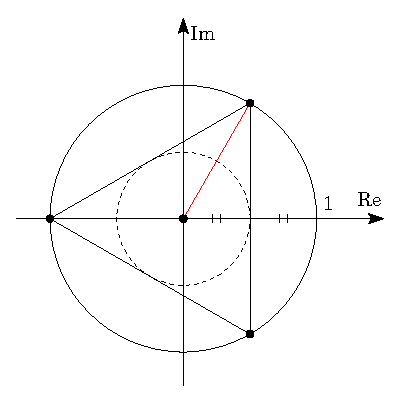
\includegraphics[width=0.25\textwidth]{AL1S1_HW_1.eps}
		\label{1_1}
		\caption{Построение фигуры.}
	\end{figure}
	Таким образом, одним из чисел является $z = -1$. Поскольку радиус вписанной окружности равен половине радиуса описанной для правильного треугольника, то координата точек на вещественной оси будет равна $\tfrac{1}{2}$. Координаты на мнимой прямой найдем из теоремы Пифагора:
	$$
		z = \dfrac{1}{2} + iy, \, y^2 = 1 - \dfrac{1}{4} = \dfrac{3}{4} \Rightarrow y = \pm \dfrac{\sqrt{3}}{2} \Rightarrow z = \dfrac{1}{2}\pm \dfrac{\sqrt{3}}{2}i
	$$
\end{proof}

\begin{problem}(\textbf{К24.6} дмн))
	Изобразить на плоскости множество точек, соответствующих комплексным числам $z$, удовлетворяющим условиям:\\
	д) $|z + 3 + 4i| \leq 5$;\\
	м) $|\RE(z) + \IM(z)| < 1$;\\
	н) $|z-1| + |z +1| = 3$;
\end{problem}
\begin{proof}
	д) Получится круг с центом в точке $-3 - 4i$ радиуса $5$:
	\begin{figure}[H]
		\centering
		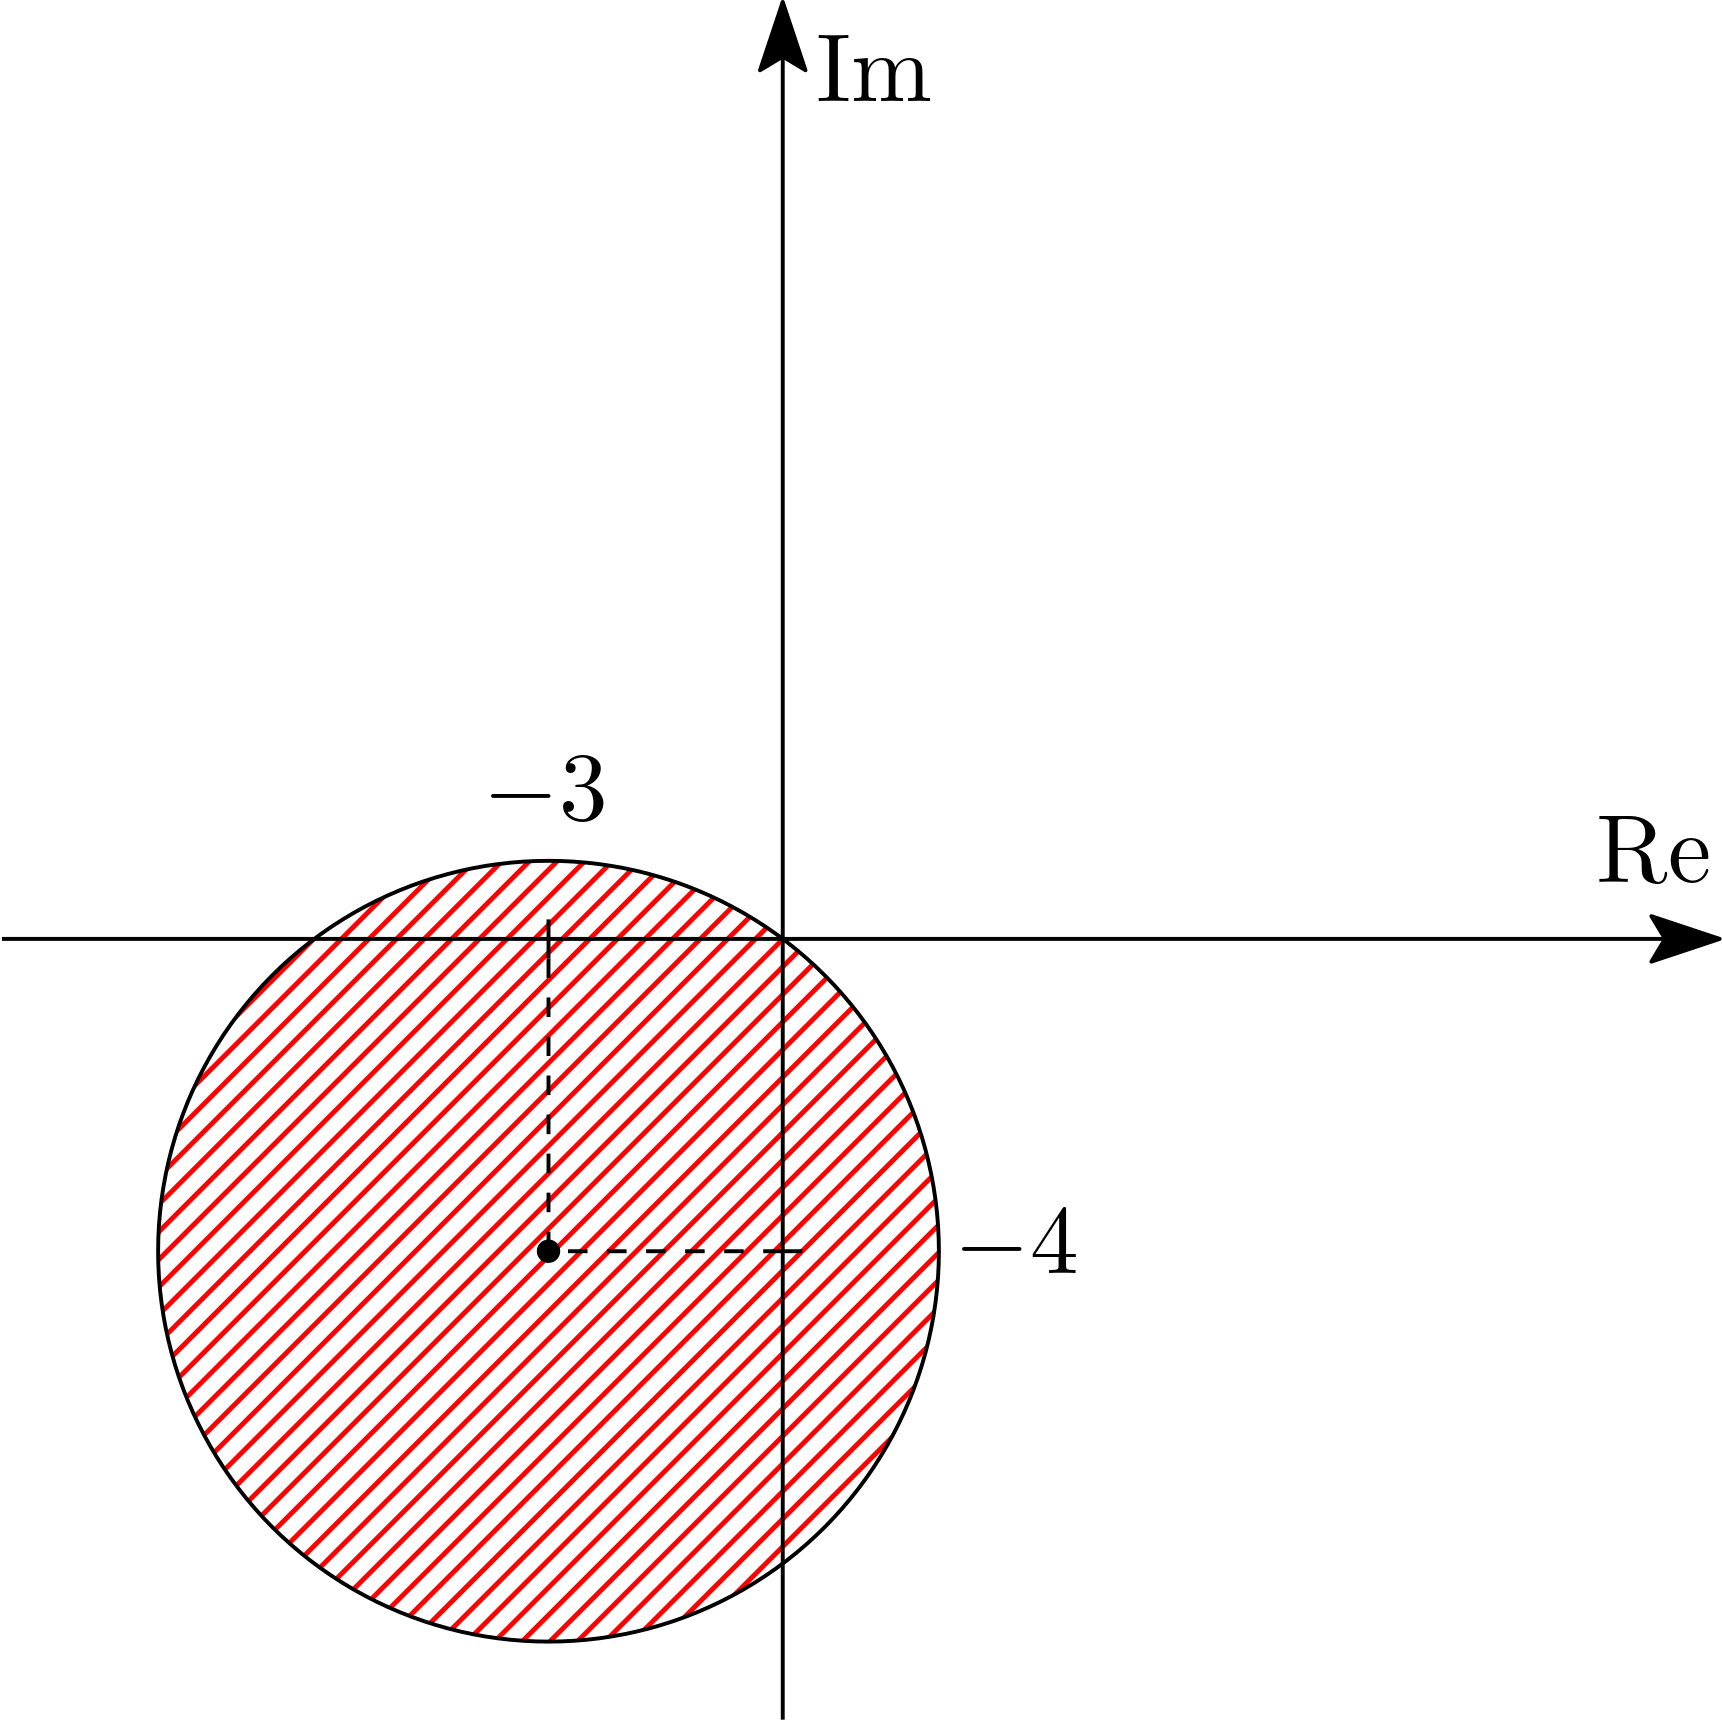
\includegraphics[width=0.3\textwidth]{AL1S1_HW_2.png}
		\label{1_2}
		\caption{Круг с центром в $-3-4i$ радиуса $5$.}
	\end{figure}
	м) Получится область плоскости, где реальная и мнимая части отличаются друго от друга не больше, чем на $1$, не включая границы $\Rightarrow$ область ограниченная прямыми $y = 1 - x$ и $y = x -1$, не включая границы:
	\begin{figure}[H]
		\centering
		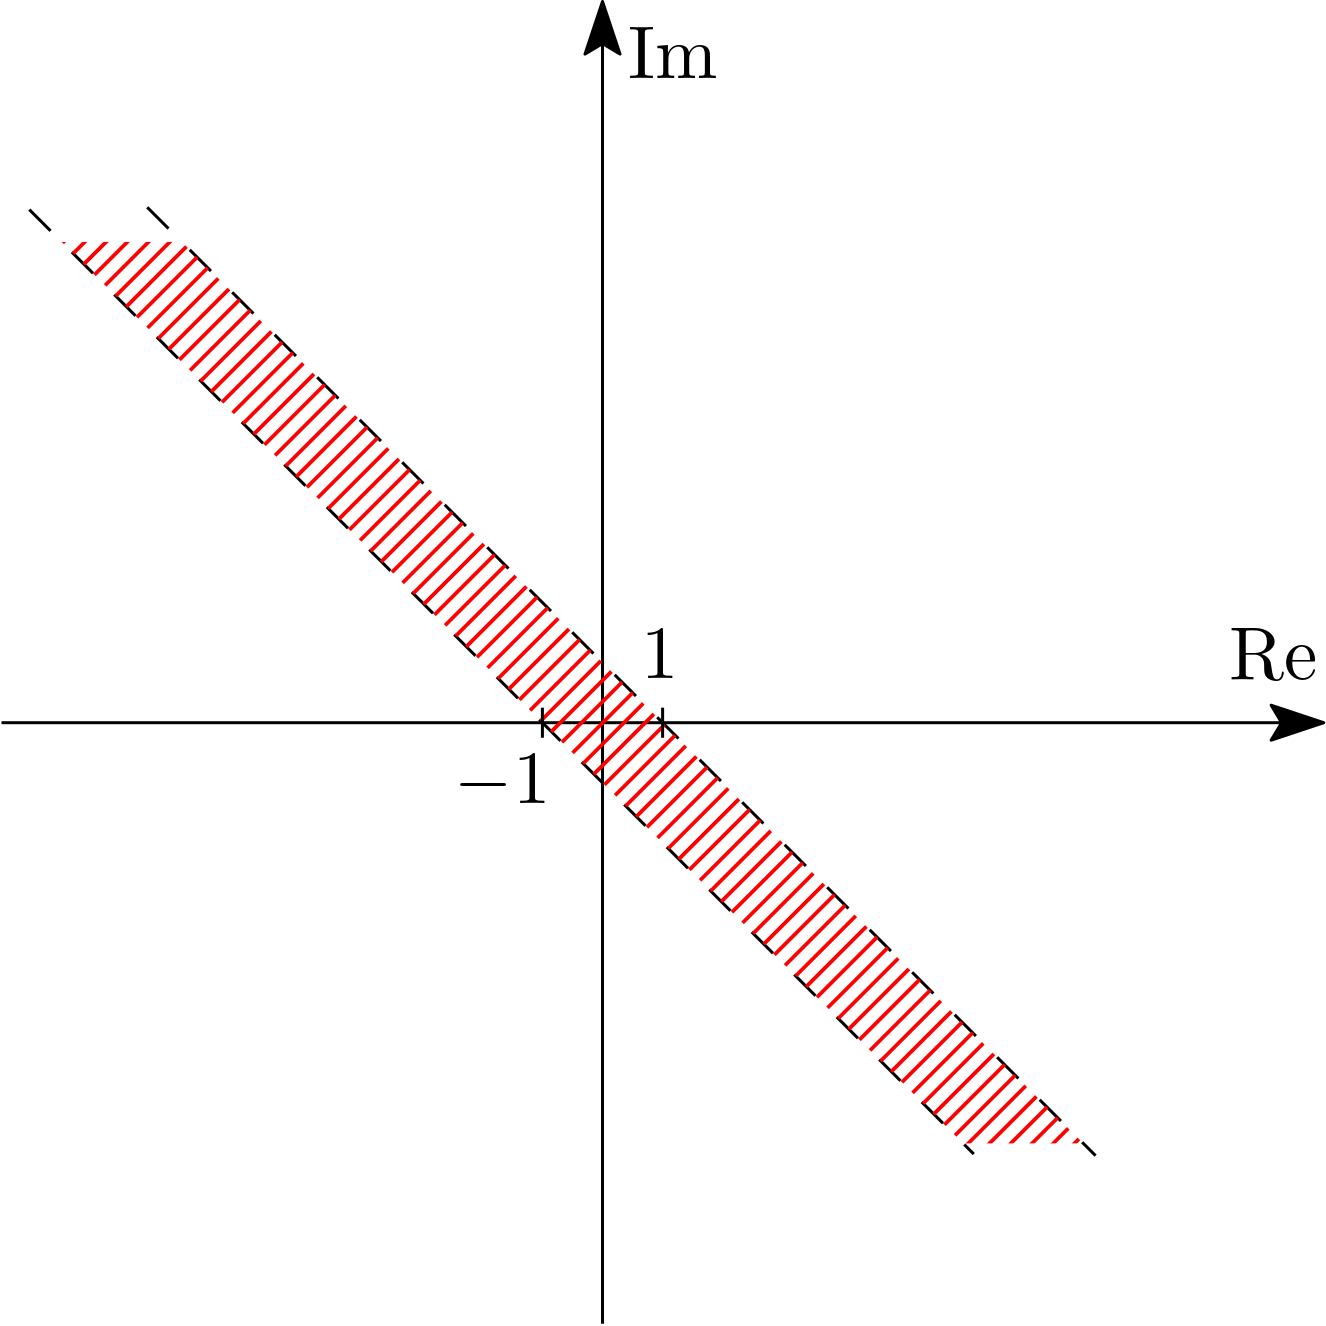
\includegraphics[width=0.35\textwidth]{AL1S1_HW_3.png}
		\label{1_3}
		\caption{Область плоскости.}
	\end{figure}
	н) Это эллипс с фокусами в точках $-1$ и $1$, $a = \dfrac{3}{2}$, $e = \dfrac{c}{a} = \dfrac{1}{\tfrac{3}{2}} = \dfrac{2}{3}$, $b = \dfrac{3}{2}\sqrt{1- \dfrac{4}{9}} = \dfrac{\sqrt{5}}{2} \Rightarrow$ получим эллпис с канонической формой записи для $z = x + iy$ в следующем виде:
	$$
		\dfrac{4x^2}{9} + \dfrac{4y^2}{5} = 1
	$$
	\begin{figure}[H]
		\centering
		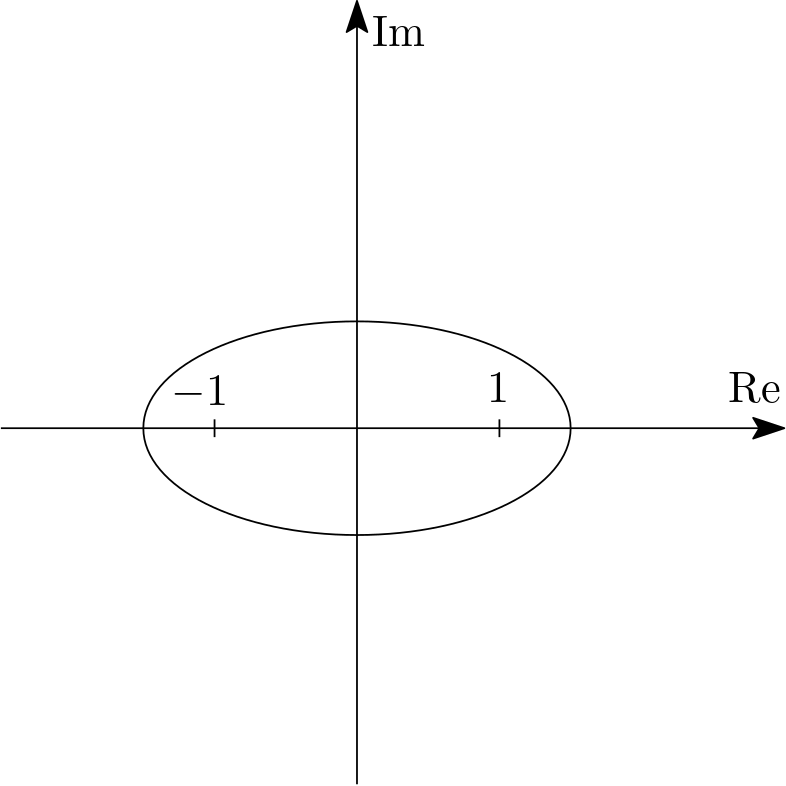
\includegraphics[width=0.35\textwidth]{AL1S1_HW_4.png}
		\label{1_4}
		\caption{Эллипс.}
	\end{figure}
\end{proof}


\end{document}